
% This LaTeX was auto-generated from MATLAB code.
% To make changes, update the MATLAB code and republish this document.

\documentclass{article}
\usepackage{graphicx}
\usepackage{color}

\sloppy
\definecolor{lightgray}{gray}{0.5}
\setlength{\parindent}{0pt}

\begin{document}

    
    
\subsection*{Contents}

\begin{itemize}
\setlength{\itemsep}{-1ex}
   \item figure 1: Default case
   \item figure 2: Wind sweep:
   \item figure 3: Wind sweep with distance:
   \item figure 4: Altitude change
   \item figure 5: part f, vary initial speed and mass so that its constrained by kinetic energy
\end{itemize}
\begin{verbatim}
% Contributors: Nathaniel Mueller
% Course number: ASEN 3801
% File name: main.m
% Created: 1/13/2026

%housekeeping
clear; clc; close all;

%increase the font sizes for document readability
set(groot, 'defaultAxesFontSize', 16);
set(groot, 'defaultTextFontSize', 16);

%givens
m = 0.05; % kg
Cd = 0.6; % coefficient of drag
g = 9.81; % acceleration due to gravity (m/s^2)
diameter = 0.02; % (m)
A = pi*(diameter/2)^2; % cross-sectional area (m^2)
h = 1655; %altitude (m)
%
rho = stdatmo(h); % density (kg/m^3)
h_vec = [0, 1600, 3200, 4800, 6400]' ; %varying altitude (m)
rho_vec = stdatmo(h_vec)' ;

%time
tspan = [0 20]; % range of time were observing (s)


%initial conditions
p_0 = [0 0 0]' ; % (m)
v_0 = [0 20 -20]' ; % (m/s)

%tolerances
T_a = 1e-8;
T_r = 1e-8;

opts = odeset('events', @hitGroundEvent, 'RelTol', T_r, 'AbsTol', T_a);
%initial condions and velocities
x0 = [p_0; v_0 ];
\end{verbatim}


\subsection*{figure 1: Default case}

\begin{verbatim}
wind_default = [0 0 0]' ; % default v = 0 wind

figure(1); hold on;

[t, x] = ode45(@(t,x) objectEOM(t,x,rho,Cd,A,m,g,wind_default), tspan, x0, opts);

plot3(x(:,1), x(:,2), -x(:,3), 'LineWidth',1.5);
xlabel('X (m)'); ylabel('Y (m)'); zlabel('Z (m)');
grid("on")
title('Default Trajectory of Sphere in Air with no Wind')
exportgraphics(gcf, 'default.png', 'Resolution', 300);
hold off;
\end{verbatim}

        \color{lightgray} \begin{verbatim}Warning: Exported image displays axes toolbar. To remove axes toolbar from
image, export again. 
\end{verbatim} \color{black}
    
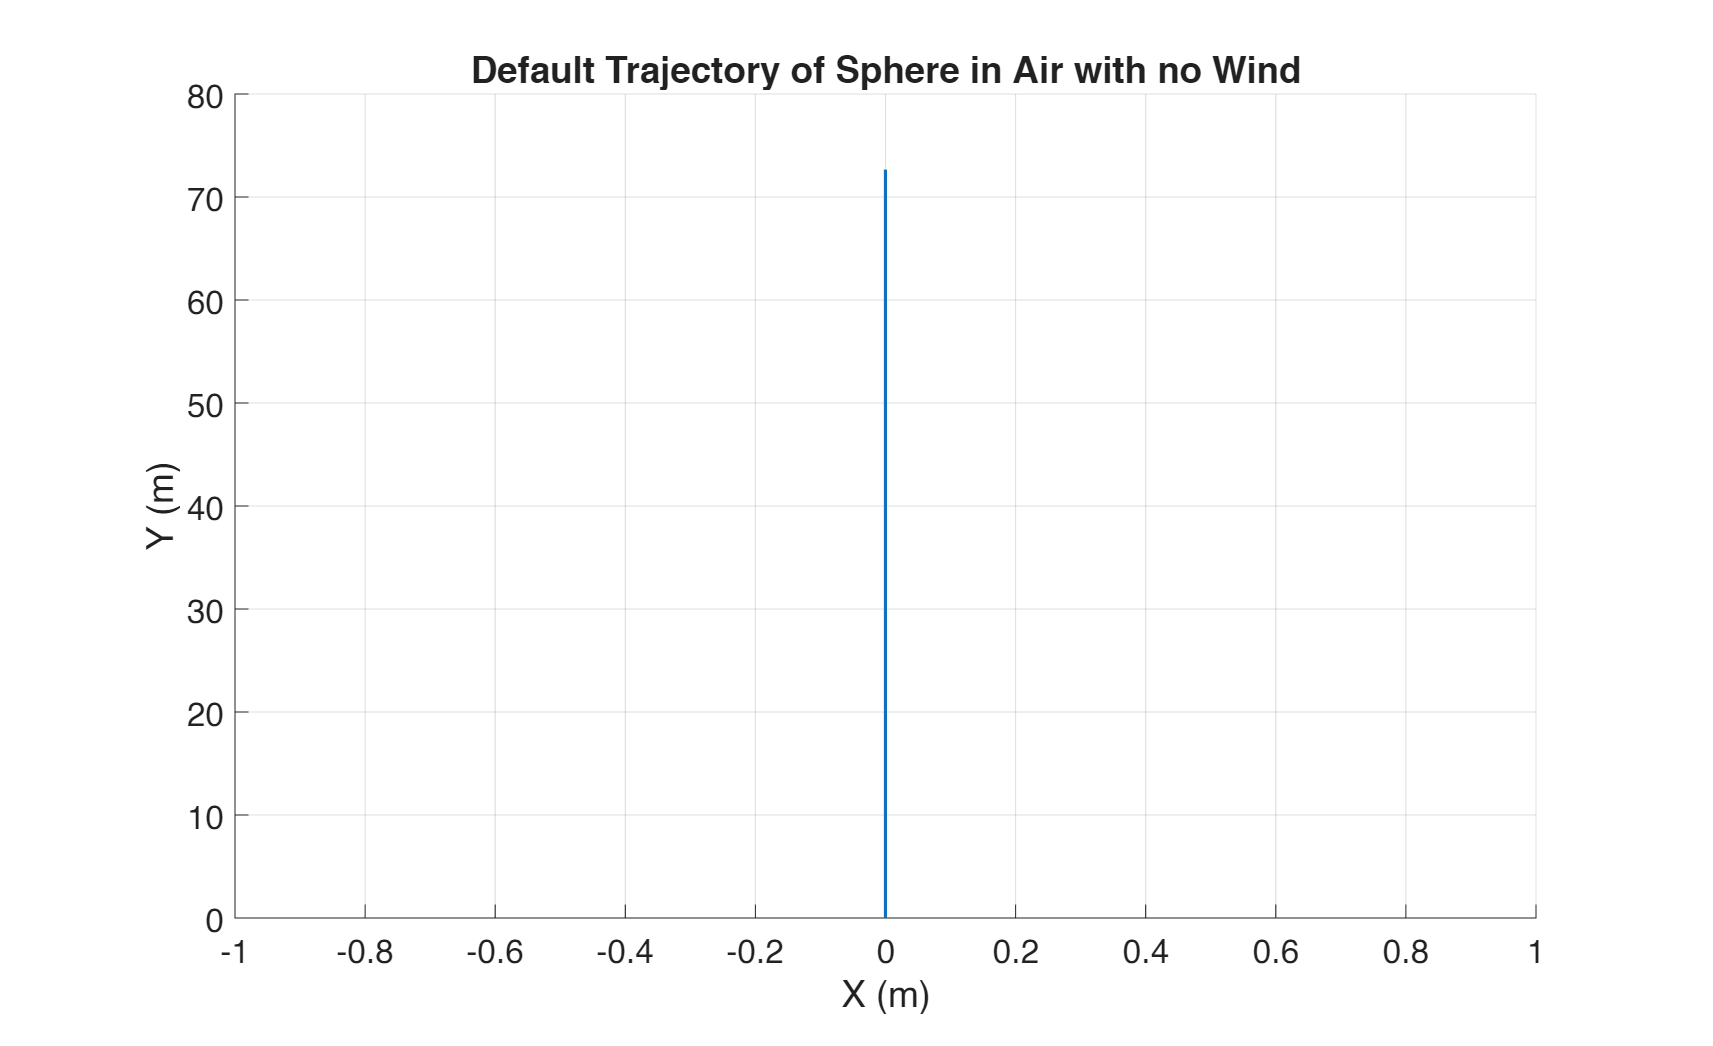
\includegraphics [width=4in]{main_01.eps}


\subsection*{figure 2: Wind sweep:}

\begin{verbatim}
%tested wind velocities, commented for later use
wind_vel = [0 0 0; 5 0 0;10 0 0; 15 0 0;20 0 0]'; % x
% wind_vel = [0 0 0; 0 5 0;0 10 0; 0 15 0;0 20 0]'; % y
% wind_vel = [ 0 0 0; 0 0 5; 0 0 10; 0 0 15; 0 0 20]'; %  z
labels = strings(1, size(wind_vel,2));

figure(2); hold on;
for h_idx = 1:size(wind_vel,2)
    [t, x] = ode45(@(t,x) objectEOM(t,x,rho,Cd,A,m,g,wind_vel(:,h_idx)), tspan, x0, opts);

    %plotting
    plot3(x(:,1), x(:,2), -x(:,3), 'LineWidth',1.5);
    labels(h_idx) = sprintf('$w = %.1f\\,i\\ \\mathrm{m/s},\\ \\frac{h}{v}=%.3f\\ \\frac{\\mathrm{m}}{\\mathrm{m/s}}$', wind_vel(1,h_idx), -x(end,1)/wind_vel(1,h_idx));
end
xlabel('X (m)'); ylabel('Y (m)'); zlabel('Z (m)');
grid("on")
legend(labels, 'Interpreter','latex', 'Location', 'best');
title('Trajectory of Sphere in Air with Wind Shear in +X')
exportgraphics(gcf, 'windShear.png', 'Resolution', 300);
hold off;


% legend('w = 0j m/s', 'w = 5j m/s', 'w = 10j m/s', 'w = 15j m/s', 'w = 20j m/s');
% exportgraphics(figure(1), 'vary_wind_y.png', 'Resolution', 300);

% legend('w = 0k m/s', 'w = -5k m/s', 'w = -10k m/s', 'w = -15k m/s', 'w = -20k m/s');
% exportgraphics(figure(1), 'vary_wind_z.png', 'Resolution', 300);
\end{verbatim}

        \color{lightgray} \begin{verbatim}Warning: Exported image displays axes toolbar. To remove axes toolbar from
image, export again. 
\end{verbatim} \color{black}
    
\includegraphics [width=4in]{main_02.eps}

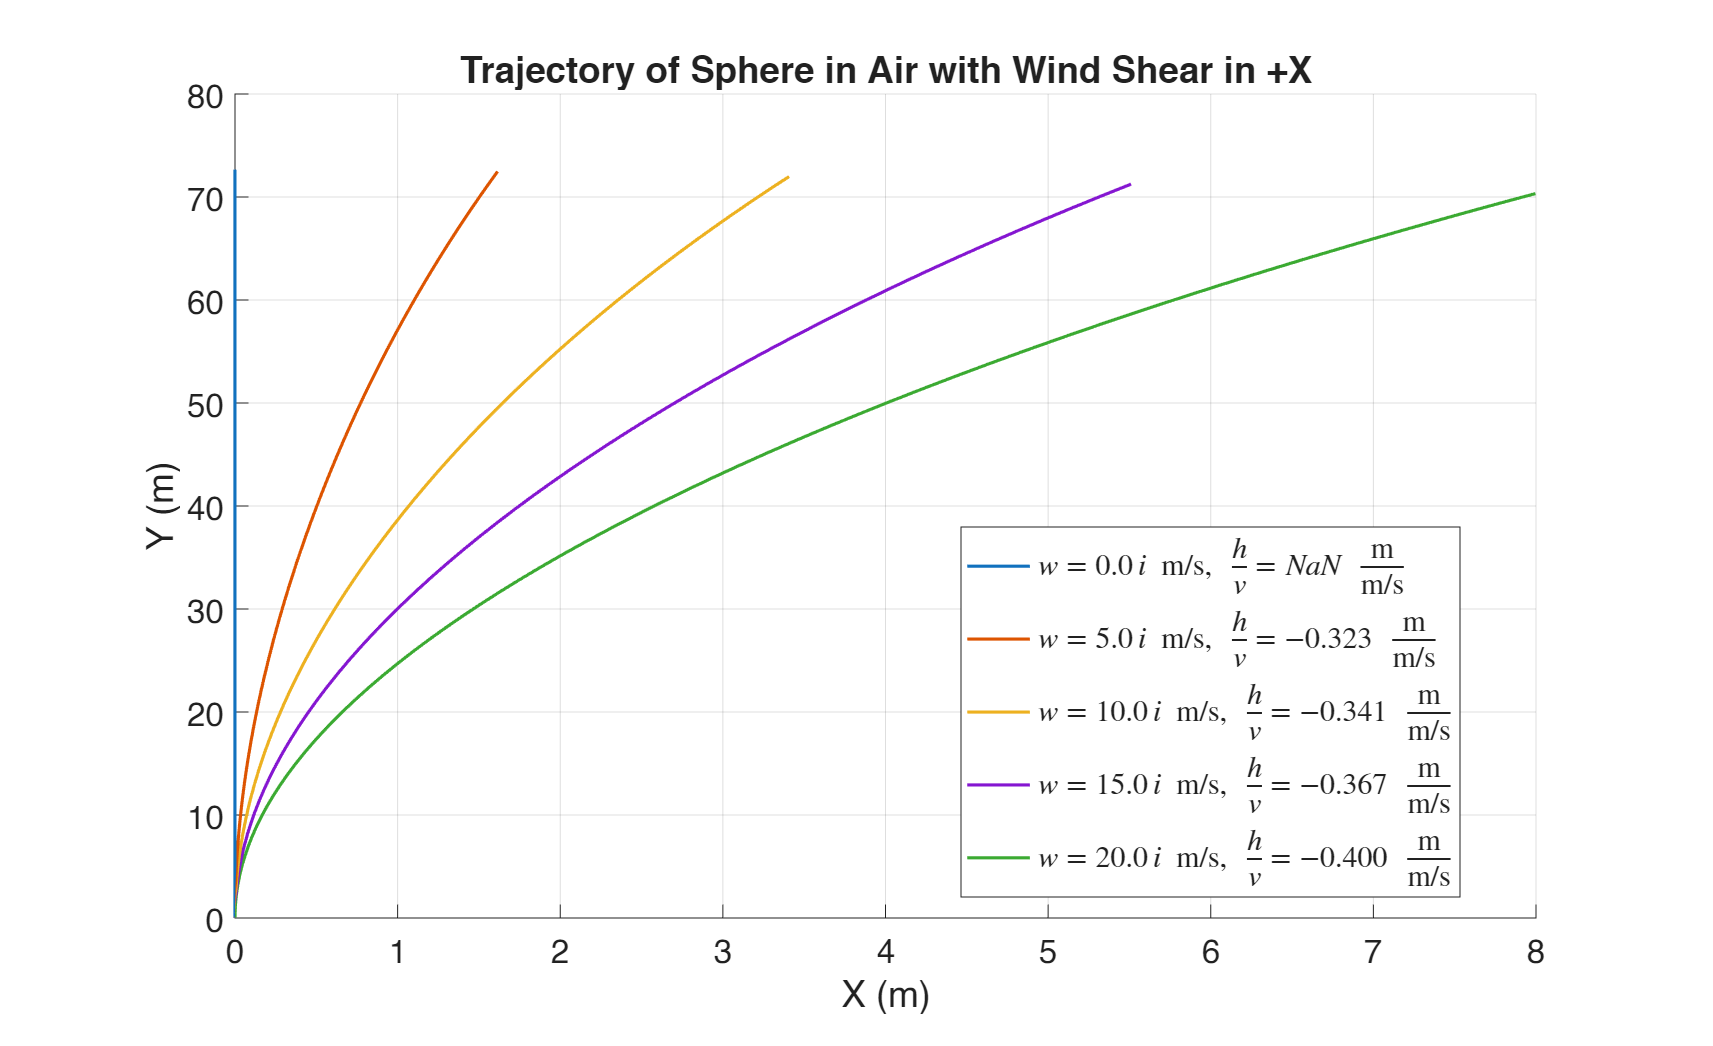
\includegraphics [width=4in]{main_03.eps}


\subsection*{figure 3: Wind sweep with distance:}

\begin{verbatim}
%tested wind velocities, commented for later use
wind_vel = [0 0 0; 5 0 0;10 0 0; 15 0 0;20 0 0]'; % x
% wind_vel = [0 0 0; 0 5 0;0 10 0; 0 15 0;0 20 0]'; % y
% wind_vel = [ 0 0 0; 0 0 5; 0 0 10; 0 0 15; 0 0 20]'; %  z
labels = strings(1, size(wind_vel,2));

figure(3); hold on;
for h_idx = 1:size(wind_vel,2)
    [t, x] = ode45(@(t,x) objectEOM(t,x,rho,Cd,A,m,g,wind_vel(:,h_idx)), tspan, x0, opts);

    %plotting
    plot3(x(:,1), x(:,2), -x(:,3), 'LineWidth',1.5);
    norm_dist = norm(x(end,1:3));
    dist_affected = norm_dist/wind_vel(1,h_idx);
    labels(h_idx) = sprintf('$w = %.1f\\,i\\ \\mathrm{m/s},\\frac{d}{v}=%.3f\\ \\frac{\\mathrm{m}}{\\mathrm{m/s}}$', wind_vel(1,h_idx), dist_affected);
end
xlabel('X (m)'); ylabel('Y (m)'); zlabel('Z (m)');
grid("on")
legend(labels, 'Interpreter','latex', 'Location', 'best');
title('Trajectory of Sphere in Air with Wind Shear in +X')
exportgraphics(gcf, 'windShear_dist.png', 'Resolution', 300);
hold off;


% legend('w = 0j m/s', 'w = 5j m/s', 'w = 10j m/s', 'w = 15j m/s', 'w = 20j m/s');
% exportgraphics(figure(1), 'vary_wind_y.png', 'Resolution', 300);

% legend('w = 0k m/s', 'w = -5k m/s', 'w = -10k m/s', 'w = -15k m/s', 'w = -20k m/s');
% exportgraphics(figure(1), 'vary_wind_z.png', 'Resolution', 300);
\end{verbatim}

\includegraphics [width=4in]{main_04.eps}

\includegraphics [width=4in]{main_05.eps}


\subsection*{figure 4: Altitude change}

\begin{verbatim}
figure(4); hold on;
for h_idx = 1:size(rho_vec,2)
    [t, x] = ode45(@(t,x) objectEOM(t,x,rho_vec(h_idx),Cd,A,m,g,wind_default), tspan, x0, opts);

    %plotting
    plot3(x(:,1), x(:,2), -x(:,3), 'LineWidth',1.5);

end
xlabel('X (m)'); ylabel('Y (m)'); zlabel('Z (m)');
grid("on")
legend('Altitude = 0 m', 'Altitude = 1600 m', 'Altitude = 3200 m', 'Altitude = 4800 m', 'Altitude = 6400 m');
title('Trajectory of Sphere in Air with Varying Altitudes')
exportgraphics(gcf, 'altChange.png', 'Resolution', 300);
hold off;
\end{verbatim}

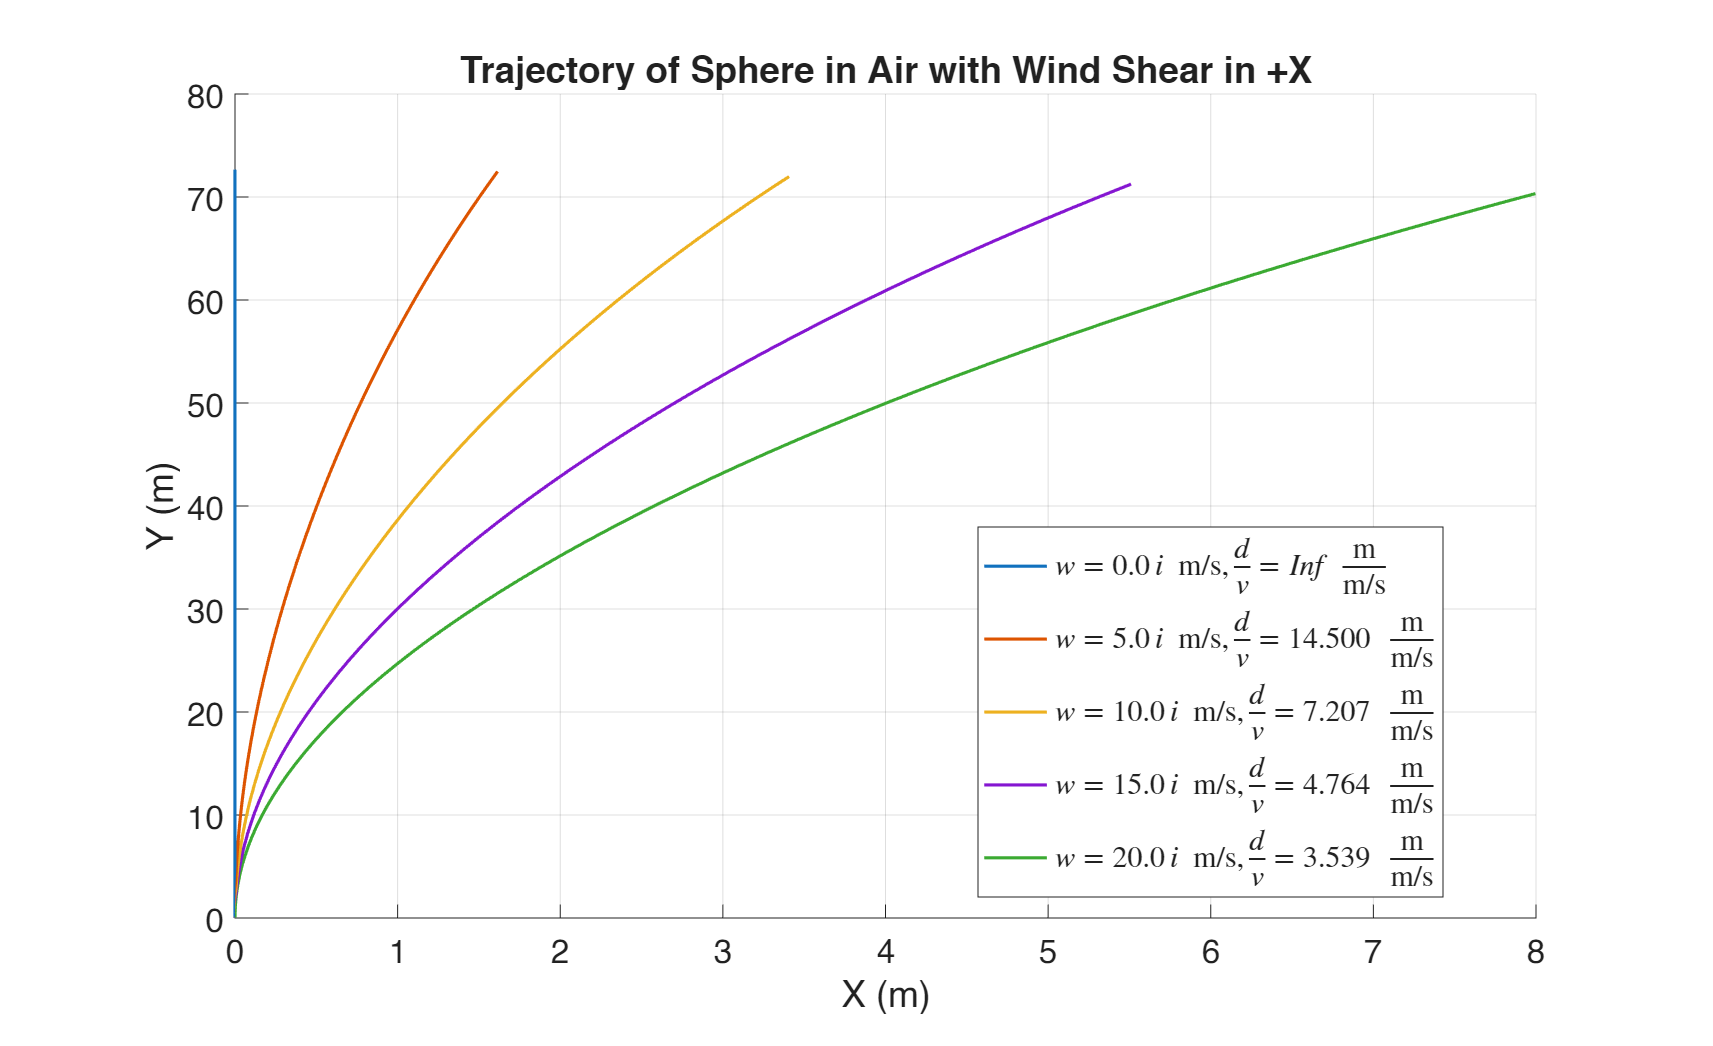
\includegraphics [width=4in]{main_06.eps}

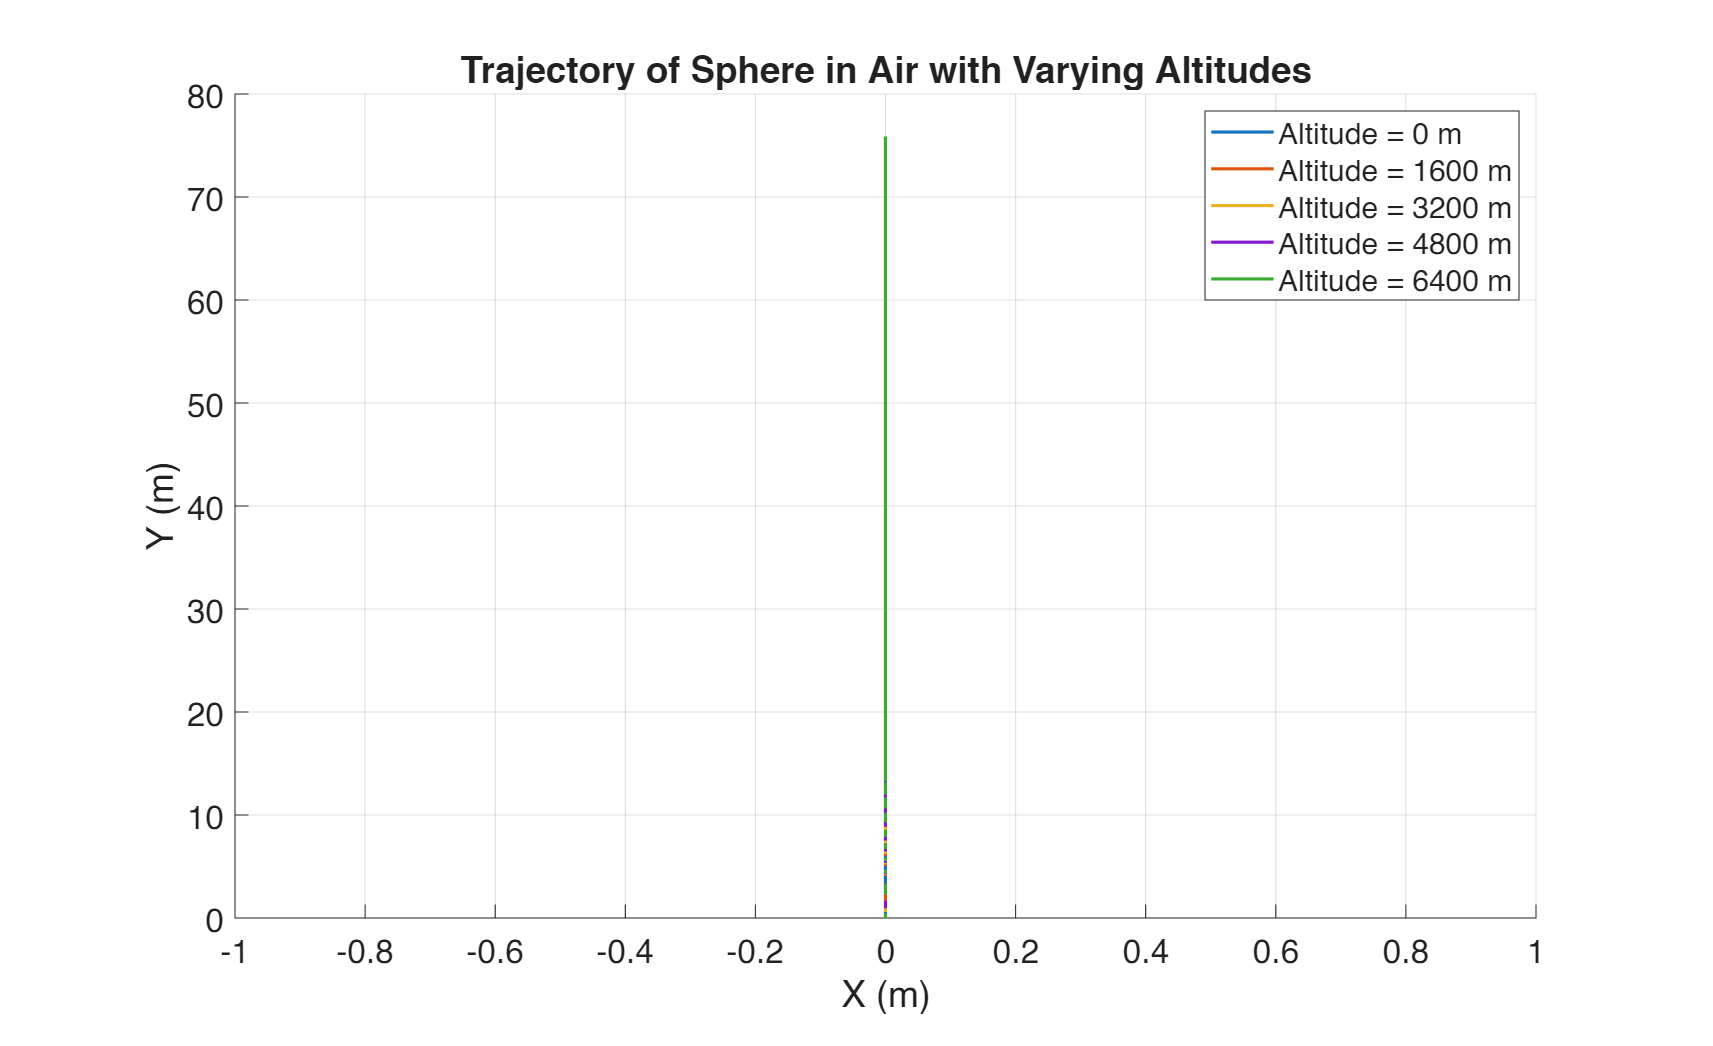
\includegraphics [width=4in]{main_07.eps}


\subsection*{figure 5: part f, vary initial speed and mass so that its constrained by kinetic energy}

\begin{par}
KE = 1/2mv\^{}2 -\ensuremath{>} v = sqrt(2KE/m) given m and KE, find v: to find v direction:
\end{par} \vspace{1em}
\begin{verbatim}
m_vec = logspace(log10(0.001), log10(0.1), 20); % (kg)
v_mag = norm(v_0); % (m/s) magnitude of the default velocity

v_dir = v_0/v_mag; % finds the unit vector of the default velocity

KE = 1/2*m*v_mag^2; % (J) finds the Kinetic energy with the default velocity and default mass

v_vec_KE_mag = sqrt(2*KE./m_vec); % finds the vector of new velocities based on the m_vec
v_vec_KE = v_vec_KE_mag.*v_dir; % puts it into 3 dimensions with unit vector (same trajectory)

N = size(m_vec,2); % number of lines produced, determined by m_vec's size
cmap = parula(N); %color map for plots

figure(5); hold on;
final_distance_pt5 = zeros(1,N);
for h_idx = 1:N
    x0 = [p_0; v_vec_KE(:,h_idx) ];
    [t, x] = ode45(@(t,x) objectEOM(t,x,rho,Cd,A,m_vec(h_idx),g,wind_default), tspan, x0, opts);
    final_distance_pt5(h_idx) = norm(x(end,2:3));
    %plotting
    plots_pt5(h_idx) = plot3(x(:,1), x(:,2), -x(:,3), 'LineWidth',1.5, 'Color', cmap(h_idx,:));

end

xlabel('X (m)'); ylabel('Y (m)'); zlabel('Z (m)');
grid("on")
legend([plots_pt5(1), plots_pt5(end)], {'m = 0.001 kg', 'm = 0.1 kg'})
title('Trajectory of Sphere in Air with Constant Kinetic Energy (varying velocity and mass)')
exportgraphics(gcf, 'distance_3d.png', 'Resolution', 300);
hold off;

figure(6)
m_vec_g = m_vec .* 1000;
plot(m_vec_g, final_distance_pt5);
xlabel('m (g)'); ylabel('Distance (m)');
grid("on")
title('Range Versus Mass of Sphere with Constant Kinetic Energy')
exportgraphics(gcf, 'distance_vs_mass.png', 'Resolution', 300);


% cont. various values of wind speed:

wind_speed_pt5 = [0 5 10 15 20];
N_wind = length(wind_speed_pt5);

range_vs_mass_wind = zeros(N_wind, N);

figure(7);
hold on;
cmap = parula(N_wind); %color map for plots
for w_idx = 1:N_wind
    wind_vec_pt5 = [wind_speed_pt5(w_idx) 0 0]' ;

    for h_idx = 1:N
        x0 = [p_0; v_vec_KE(:, h_idx)];
        [t, x] = ode45(@(t,x) objectEOM(t,x,rho,Cd,A,m_vec(h_idx),g,wind_vec_pt5), tspan, x0, opts);

        range_vs_mass_wind(w_idx, h_idx) = norm(x(end,1:3));
    end
    plot(m_vec*1000, range_vs_mass_wind(w_idx,:), 'LineWidth', 1.5, 'Color',cmap(w_idx,:));
end
xlabel('mass (g)'); ylabel('Absolute Range (m)');
title('Range Versus Mass of Sphere with Constant Kinetic Energy at Various Wind Speeds')
legend('w = 0i m/s', 'w = 5i m/s', 'w = 10i m/s', 'w = 15i m/s', 'w = 20i m/s');
exportgraphics(gcf, 'distance_vs_mass_vs_wind.png', 'Resolution', 300);
%hit ground event

function [position, isterminal, direction] = hitGroundEvent(t, x)
%inputs: t = time used to track when event x occurs
%        x = position matrix x being observed for when event occurs (in our
%            case the object's z position at 0
% methodology: just an event that tracks when we go up (down in our case
% because our z axis is flipped) through 0
  position = x(3); % The value that we want to be zero
  isterminal = 1;  % Halt integration
  direction = 1;   % only detect if going downwards (ie its okay if were going up from below height h to above height h)
end
\end{verbatim}

        \color{lightgray} \begin{verbatim}Warning: Exported image displays axes toolbar. To remove axes toolbar from
image, export again. 
\end{verbatim} \color{black}
    
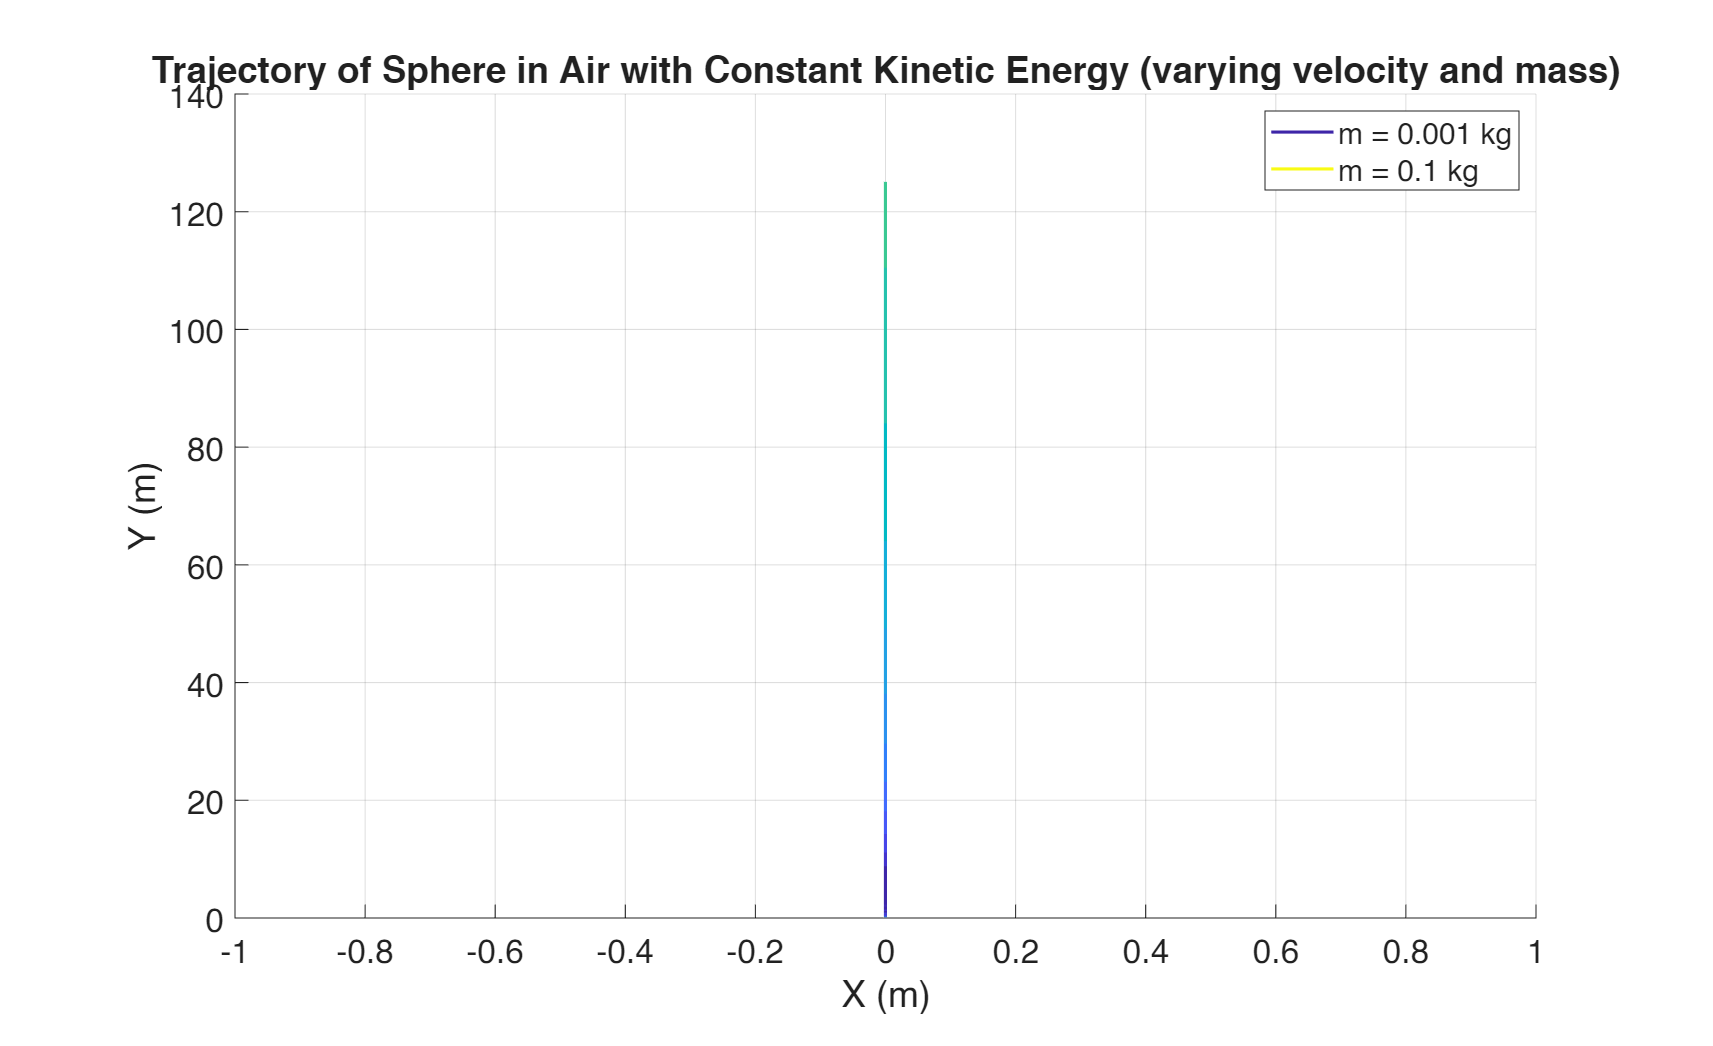
\includegraphics [width=4in]{main_08.eps}

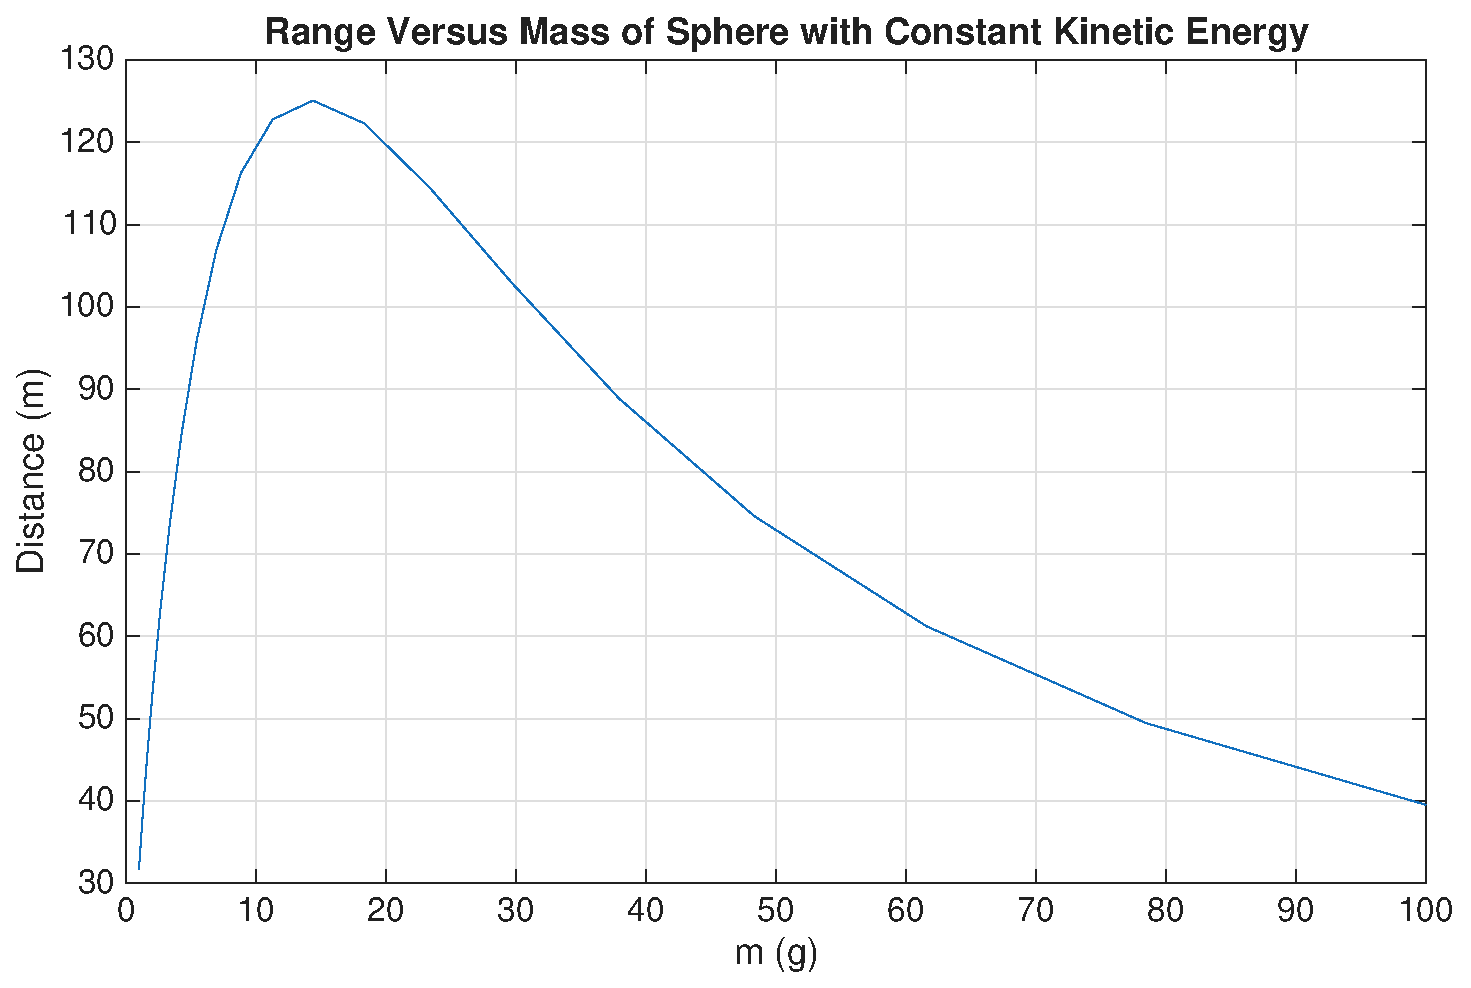
\includegraphics [width=4in]{main_09.eps}

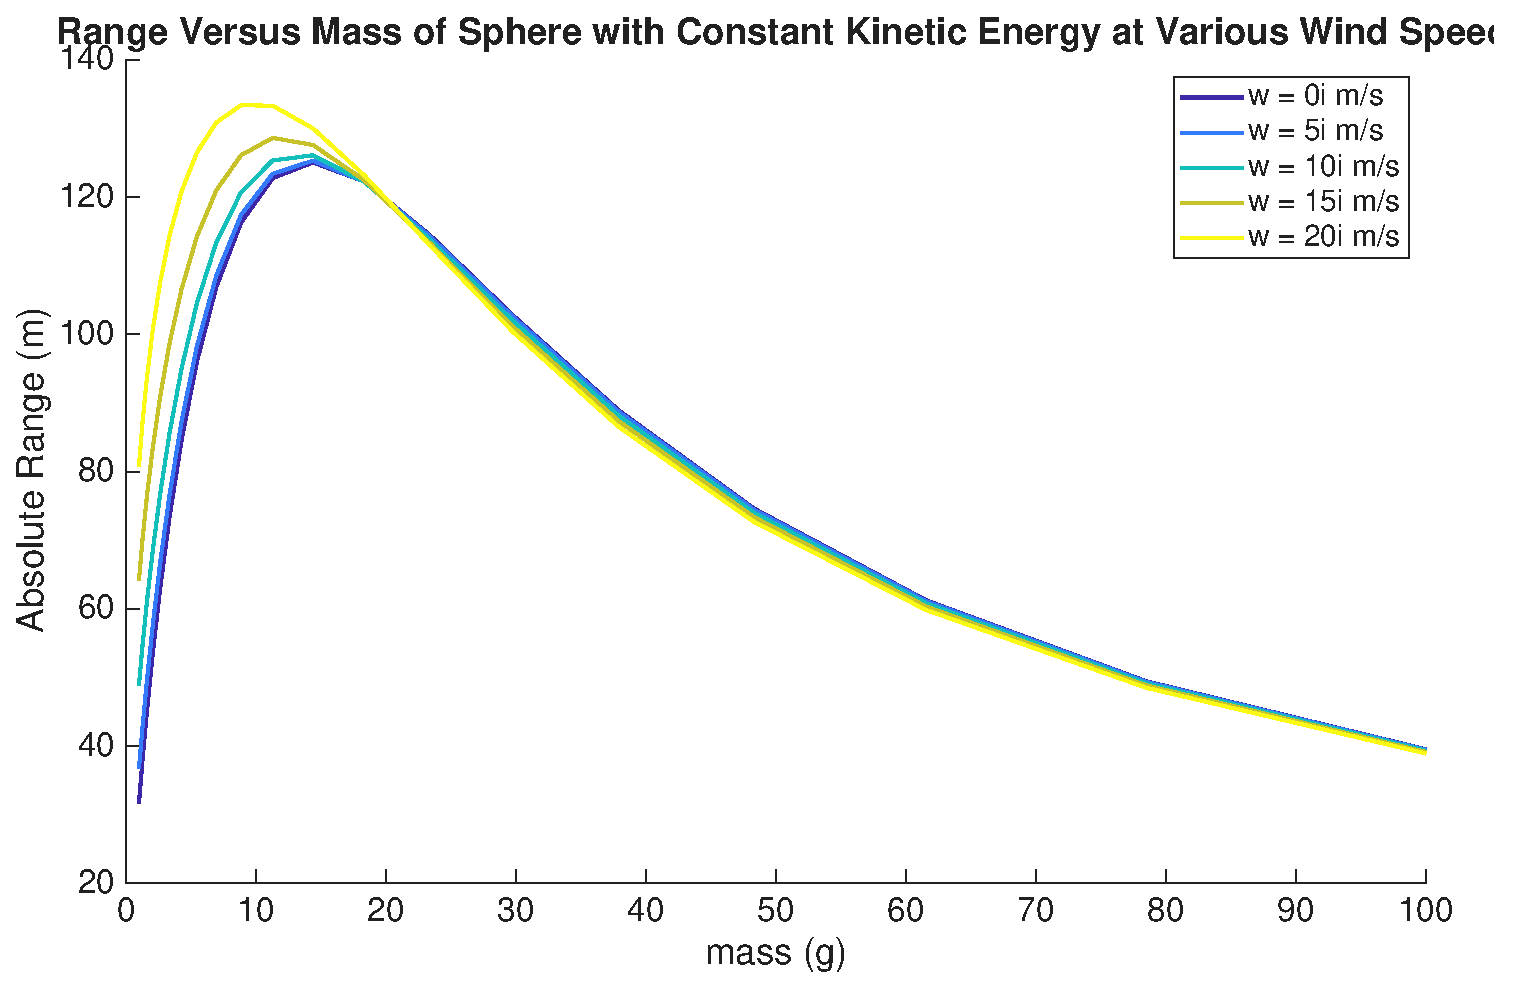
\includegraphics [width=4in]{main_10.eps}



\end{document}

